% Basic settings
\documentclass[a4paper,9pt]{article}
\usepackage[utf8]{inputenc}
\usepackage[german]{babel}

% Layout settings
\usepackage[top=1.1cm, bottom=1.5cm, left=1cm, right=1cm, headsep=5pt]{geometry}
\usepackage[compact]{titlesec}
\titlespacing{\section}{0pt}{0pt}{0pt}
\titlespacing{\subsection}{0pt}{0pt}{0pt}
\titlespacing{\subsubsection}{0pt}{0pt}{0pt}
\setlength{\parindent}{0em}
\setlength{\parskip}{1em}

% My colors
\usepackage[table,dvipsnames]{xcolor}
\definecolor{babyblue}{HTML}{A1CAF1}
\definecolor{peach}{HTML}{EFC9AF}
\definecolor{crayola}{HTML}{FFEE93}

% Custom section formatting
\newcommand{\sect}[1]{\section*{\colorbox{babyblue}{\makebox[\linewidth][l]{#1}}}}
\newcommand{\ssect}[1]{\subsection*{\colorbox{peach}{\makebox[\linewidth][l]{#1}}}}
\newcommand{\sssect}[1]{\subsubsection*{\colorbox{crayola}{\makebox[\linewidth][l]{#1}}}}

% Two columns
\usepackage{multicol}

% Colored boxes
\usepackage[most]{tcolorbox}

% A base set of colorbox that is then customised
\tcbset {
    base/.style={
        boxrule=0mm,
        leftrule=1mm,
        left=1.75mm,
        arc=0mm,
        fonttitle=\bfseries,
        colbacktitle=black!10!white,
        coltitle=black,
        toptitle=0.75mm,
        bottomtitle=0.25mm,
        title={#1}
    }
}

% Box with red line for definitions
\definecolor{bittersweet}{rgb}{1.0, 0.44, 0.37}
\newtcolorbox{definition}[1]{
    colframe=bittersweet,
    base={#1}
}

% Box with blue line for mainboxes
\definecolor{brandblue}{rgb}{0.34, 0.7, 1}
\newtcolorbox{mainbox}[1]{
    colframe=brandblue,
    base={#1}
}

% Subboxes don't have any color
\newtcolorbox{subbox}[1]{
    colframe=black!20!white,
    base={#1}
}

% Package to include images/sketches
\usepackage{graphicx}

% Mathematical typesetting & symbols
\usepackage{amsfonts}
\usepackage{amsmath}
\usepackage{amssymb}
\usepackage{amsthm}
\usepackage{bigints}
\usepackage{mathtools}
\usepackage{wasysym}
\usepackage{cancel}

% Math helper stuff
\newcommand{\N}{\mathbb{N}}
\newcommand{\Z}{\mathbb{Z}}
\newcommand{\R}{\mathbb{R}}
\newcommand{\Q}{\mathbb{Q}}
\newcommand{\E}{\mathbb{E}}
\newcommand{\F}{\mathbb{F}}
\newcommand{\V}{\mathbb{V}}
\renewcommand{\P}{\mathbb{P}}
\newcommand{\true}{\texttt{true}}
\newcommand{\false}{\texttt{false}}
\newcommand{\bigO}{\mathcal{O}}
\newcommand{\comp}{\;\circ\;}

\newcommand{\diff}[1]{\,\mathrm{d}#1}

\usepackage{enumitem}

% Draw stuff
\usepackage{tikz-cd}
\usepackage{paracol}

% Comment packages
\usepackage{verbatim}
\usepackage{comment}
\usepackage{lipsum}
\usepackage{color}

% Path to graphics
\graphicspath{{images/}}

%\includeonly{sections/approximation-durch-polynomfunktionen}

\begin{document}
    \raggedcolumns

    \section{Integrationsmethoden}\label{sec:integrationsmethoden}

\textbf{Zur Erinnerung:}

$\int x \cdot x \diff{x} = \int x^2 \diff{x} = \frac{x^3}{3} + C$

$\int x \diff{x} \cdot \int x \diff{x} = \left( \frac{x^2}{x} + C_1 \right) \left( \frac{x^2}{2} + C_2 \right) = \frac{x^4}{4} + \left( C_1 + C_2 \right) \frac{x^2}{2} + C_1 C_2$

Im Allgemeinen: $\int u(x) \cdot v(x) \diff{x} \neq \int u(x) \diff{x} \cdot \int v(x) \diff{x}$

Es gibt kein allgemeingültiges Rezept für die Berechnung der Integrale von Produkten.
Es gibt aber mehrere Integrations-Techniken, die für bestimmte Formen von Produkten (und andere Funktionstypen) zum Ziel führen.
Da die Integration die Umkehrung der Ableitung ist, könnte man versuchen, die Produkt- und die Kettenregel umzukehren.

\subsection{Integration durch Substitution}\label{subsec:integration-durch-substitution}

Diese Integrationsmethode beruht auf der Kettenregel für die Ableitung: \[F(u(x)) = \int (F(u(x)))' \diff{x} = \int F'(u) \cdot u'(x) \diff{x}\]

\begin{definition}{Rezept: Integration durch Substitution}
    \begin{enumerate}
        \item Substitutionsgleichung für $x$: $u = g(x)$
        \item Substitutionsgleichung für $\diff{x}$: $\frac{\diff{u}}{\diff{x}} = g'(x) \Rightarrow \diff{x} = \frac{\diff{u}}{g'(x)}$
        \item Integralsubstitution
        \item Integration
        \item Rücksubstitution (nur für unbestimmte Integrale)
    \end{enumerate}
\end{definition}

\textbf{Beispiel 1:} \[\int_0^{\pi / 4} \sin^2(x) \cdot \cos(x) \diff{x}\]
\begin{enumerate}
    \item Substitutionsgleichung für $x$: $u(x) = \sin(x)$
    \item Substitutionsgleichung für $\diff{x}$: $\frac{\diff{u}}{\diff{x}} = \cos(x) \Rightarrow \diff{x} = \frac{\diff{u}}{\cos(x)}$
    \item Integralsubstitution: $\int_{0}^{\pi / 4} \sin^2(x)\cos(x) \diff{x} = \int_{0}^{\sqrt{2}/2} u^2 \cdot \cos(x) \cdot \frac{\diff{u}}{\cos(x)} = \int_{0}^{\sqrt{2} / 2} u^2 \diff{u}$
    \item Integration: $\int_{0}^{\sqrt{2} / 2} u^2 \diff{u} = \left[ \frac{u^3}{3} \right]_{0}^{\sqrt{2}/2} = \frac{1}{3} \left( \frac{\sqrt{2}}{2} \right)^3 \approx 0.12$
\end{enumerate}

\textbf{Beispiel 2:} \[ \int \frac{6x^2 - 12}{x^3 - 6x + 1} \diff{x} = \int (6x^2 - 12) \cdot (x^3 - 6x + 1)^{-1} \diff{x} \]
\begin{enumerate}
    \item Substitutionsgleichung für $x$: $u(x) = x^3 - 6x + 1$
    \item Substitutionsgleichung für $\diff{x}$: $\frac{\diff{u}}{\diff{x}} = 3x^2 - 6 \Rightarrow \diff{x} = \frac{\diff{u}}{3x^2 - 6}$
    \item Integralsubstitution: $\int (6x^2 - 12)(x^3 - 6x + 1)^{-1} \diff{x} = \int (6x^2 -12) \cdot u^{-1} \cdot \frac{\diff{u}}{3x^2 - 6} = 2 \cdot \int \frac{1}{u} \diff{u}$
    \item Integration: $2 \cdot \int \frac{1}{u} \diff{u} = 2 \cdot (\ln |u| + C) = 2 \ln |u| + \tilde{C} \;\;\;\; (\tilde{C} = 2C)$
    \item Rücksubstitution: $2 \ln |u| + \tilde{C} = 2 \ln |x^3 - 6x + 1| + \tilde{C}$
    \item Kontrolle: $(2 \ln |x^3 - 6x + 1|)' = \frac{2}{x^3 -6x + 1} \cdot (3x^3 - 6) = \frac{6x^2 - 12}{x^3 - 6x + 1}$
\end{enumerate}

\begin{subbox}{Satz}
    Für eine Funktion $f$ und Konstanten $a,b$ gilt: \[\int f(ax + b) \diff{x} = \frac{1}{a} \cdot F(ax + b)\]
\end{subbox}

\textbf{Beispiel:} $\int \cos(5x + 7) \diff{x}$

$f(u) = \cos(u)$, $a = 5$, $b = 7$, $F(u) = \sin(u)$

Somit ist: $\int \cos(5x + 7) \diff{x} = \frac{1}{a} \cdot F(ax + b) = \frac{1}{5} \cdot \sin(5x + 7)$

\subsection{Partielle Integration}\label{subsec:partielle-integration}

Diese Integrationsmethode beruht auf der Produktregel für die Ableitung: \[ (u(x) \cdot (v(x)))' = u'(x) \cdot v(x) + u(x) \cdot v'(x) \]

Beide Seiten der Gleichung integrieren liefert: \[ \int (u(x) \cdot (v(x)))' \diff{x} = \int u'(x) \cdot v(x) + u(x) \cdot v'(x) \diff{x}\]

Die linke Seite ist gleich $u(x) \cdot v(x)$.
Die rechte Seite ist so speziell, dass Integrale dieser Form wohl nur sehr selten auftreten.
Wir können den entsprechenden Ausdruck jedoch als Summe von zwei Integralen schreiben - die einzelnen Integrale sind nun nicht mehr ganz so exotisch.
Dies führt zur Gleichung \[ u(x) \cdot v(x) = \int u'(x) \cdot v(x) \diff{x} + \int u(x) \cdot v'(x) \diff{x} \]
Auflösen nach einem der beiden Integrale ergibt die Formel:
\begin{definition}{Partielle Integration (Unbestimmte Integrale)}
    \[\int u(x) \cdot v'(x) \diff{x} = u(x) \cdot v(x) - \int u'(x) \cdot v(x) \diff{x}\]
\end{definition}

\textbf{Beispiel:} $\int x \cdot e^x \diff{x}$
\begin{multicols}{2}
    \begin{itemize}[label={}]
        \item $u(x) = x$
        \item $v'(x) = e^x$
        \item $u'(x) = 1$
        \item $v(x) = e^x$
    \end{itemize}
\end{multicols}
$\int x \cdot e^x \diff{x} = x \cdot e^x - \int 1 \cdot e^x \diff{x} = x \cdot e^x - e^x + C = (x - 1)e^x + C$

Die oben hergeleitete Formel lässt sich auch auf bestimmte Integrale anwenden:
\begin{definition}{Partielle Integration (Bestimmte Integrale)}
    \[ \int_{a}^{b} u(x) \cdot v'(x) \diff{x} = \left[ u(x) \cdot v(x) \right]_{a}^{b} - \int_{a}^{b} u'(x) \cdot v(x) \diff{x}\]
\end{definition}

\subsection{Integration durch Partialbruchzerlegung}\label{subsec:integration-durch-partialbruchzerlegung}

Diese Methode ist auf die Integration von \emph{echt gebrochenrationalen} Funktionen zugeschnitten. \[ f(x) = \frac{g(x)}{h(x)} = \frac{a_m x^m + a_{m-1} x^{m-1} + \dots + a_1 x + a_0}{b_n x^n + b_{n-1} x^{n-1} + \dots + b_1 x + b_0} \;\;\;\; \text{mit $m < n$}
\]

Diese Integrationsmethode besteht aus zwei Teilen: \textbf{Partialbruchzerlegung} und \textbf{Integration der Partialbrüche}.

\begin{definition}{Rezept: Integration durch Partialbruchzerlegung}
    I Partialbruchzerlegung
    \begin{enumerate}
        \item Reelle Nullstellen des Nenners $h(x)$ mit Multiplizitäten bestimmen
        \item Jeder dieser Nullstellen wird eine Summe von Brüchen zugeordnet:
        \begin{align*}
            &x_1 \text{ist einfache Nullstelle} \rightarrow \frac{A}{x - x_1} \\
            &x_1 \text{ist doppelte Nullstelle} \rightarrow \frac{A_1}{x - x_1} + \frac{A_2}{(x - x_1)^2} \\
            &x_1 \text{ist $r$-fache Nullstelle} \rightarrow \frac{A_1}{x - x_1} + \frac{A_2}{(x - x_1)^2} + \dots + \frac{A_r}{(x - x_1)^r}
        \end{align*} $A_1$, $A_2$, $\dots$, $A_r$ sind (zunächst noch unbekannte) reelle Konstanten.
        \item $f(x)$ wird mit der Summe aller Partialbrüche gleichgesetzt.
        \item Bestimmung der Konstanten $A$, $A_1$, $A_2$, \dots, $A_r$, etc.
        \begin{enumerate}
            [label=(\roman*)]
            \item Alle Brüche auf einen gemeinsamen Nenner bringen.
            \item Durch Einsetzen von $x$-Werten (z.B.\ Nullstellen der entsprechenden Polynome) erhält man ein lineares Gleichungssystem.
            \item Gleichungssystem lösen (z.B.\ mit Gauss-Algorithmus)
        \end{enumerate}
    \end{enumerate}
    II Integration der Partialbrüche
    \begin{align*}
        \int \frac{1}{x - x_0} \diff{x} &= \ln |x - x_0| + C \\
        \int \frac{1}{(x - x_0)^r} \diff{x} &= \frac{1}{(1 - r)(x - x_0)^{r-1}} + C
    \end{align*}
\end{definition}

\textbf{Beispiel:}
Bestimmen Sie $\int \frac{2x^3 - 14x^2 + 14x + 30}{x^2 - 4} \diff{x}$

Die Funktion im Integral ist \textbf{unecht gebrochen rational}.

\begin{itemize}
    \item Umformung mithilfe von Polynomdivision: \[(2x^3 - 14x^2 + 14x + 30) : (x^2 - 4) = 2x - 14 + \frac{22x - 26}{x^2 - 4}\]
    \item I Partialbruchzerlegung des echt gebrochenen rationalen Teils:
    \begin{enumerate}
        \item Nullstellen vom Nenner: $x_1 = 2$, $x_2 = -2$
        \item Partialbruchzerlegung: $x_1 \rightarrow \frac{A}{x-2}$, $x_2 \rightarrow \frac{B}{x+2}$
        \item Gleichsetzen: $\frac{22x - 26}{x^2 -4} = \frac{A}{x - 2} + \frac{B}{x + 2} \left( = \frac{A(x + 2) + B(x - 2)}{(x-2)(x+2)} \right)$ \\ $x = 2$ einsetzen: $18 = 4A \Rightarrow A = 4.5$ \\ $x = -2$ einsetzen: $-70 = -4B \Rightarrow B = 17.5$ \\ Somit: $\frac{22x - 26}{x^2 - 4} = \frac{4.5}{x - 2} + \frac{17.5}{x + 2}$
    \end{enumerate}
    \item II Integration:
    \begin{align*}
        \int \frac{2x^3 - 14x^2 + 14x + 30}{x^2 - 4}\diff{x} &= \int 2x - 14 + \frac{4.5}{x - 2} + \frac{17.5}{x + 2} \diff{x} \\
        &= x^2 - 14x + 4.5 \ln |x - 2| + 17.5 \ln |x + 2| + C
    \end{align*}
\end{itemize}

\textbf{WICHTIG:} Die Partialbruchzerlegung funktioniert für \textcolor{red}{echt gebrochen rationale} Funktionen.
Falls die gegebene Funktion dieses Kriterium nicht erfüllt, wird vorgängig eine Polynomdivision benötigt.

    \newpage

    \section*{Serie 2}

    \subsection*{Aufgabe 1}

    a) Es gibt $2^{15} \cdot (2^6 - 1) = 2064384$ Möglichkeiten.

    b) Die Maschinengenauigkeit ist $5 \cdot 10^{-16}$.

    c) Die erste Rechenmaschine hat eine Genauigkeit von $2^{-53}$.
    Die zweite Rechenmaschine dagegen hat eine Genauigkeit von $16^{-14}$.
    Daher ist die zweite Rechenmaschine ist genauer.

    \newpage

    \section{Uneigentliche Integrale}\label{sec:uneigentliche-integrale}

Ein \textbf{uneigentliches Integral} hat die Eigenschaft, dass der Integrationsbereich unendlich gross ist oder eine Polstelle enthält.

\subsection{Uneigentlicher Integrationsbereich}\label{subsec:uneigentlicher-integrationsbereich}

\begin{definition}{Definition}
    \begin{multicols}{2}
        \[\int_{a}^{\infty} f(x) \diff{x} = \lim_{t \rightarrow \infty} \int_{a}^{t} f(x) \diff{x}\] Dieses ``uneigentliche Integral'' existiert also, wenn der Grenzwert auf der rechten Seite der obigen Gleichung existiert.

        \begin{center}
            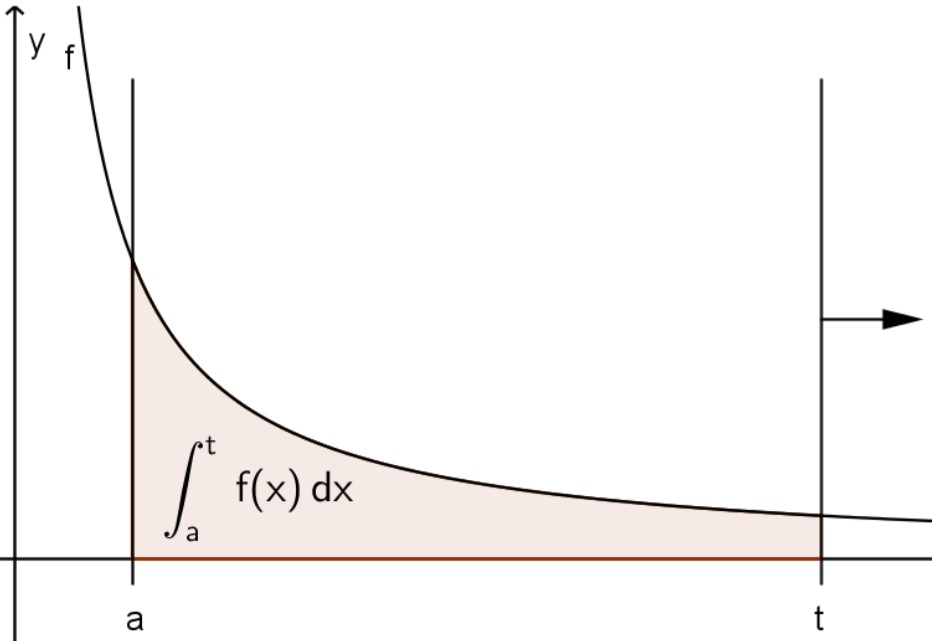
\includegraphics[scale=0.2]{uneigentlicher-integral}
        \end{center}
    \end{multicols}
\end{definition}

\textbf{Bemerkung:} Für die untere Grenze gilt entsprechend: $\int \limits_{-\infty}^{b} f(x) \diff{x} = \lim \limits_{t \rightarrow -\infty} \int \limits_{t}^{b} f(x) \diff{x}$

\textbf{Beispiele:}
\begin{multicols}{2}
    \begin{itemize}
        \item $\int \limits_{1}^{\infty} \frac{1}{x^2} \diff{x} \Rightarrow \int \limits_{1}^{t} \frac{1}{x^2} \diff{x} = \left[ -\frac{1}{x} \right]_{1}^{t} = -\frac{1}{t} + 1 \xrightarrow[t \to \infty]{} 1$
        \item $\int \limits_{-\infty}^{0} e^x \diff{x} \Rightarrow \int \limits_{t}^{0} e^x \diff{x} = \left[ e^x \right]_{t}^{0} = 1 - e^t \xrightarrow[t \to -\infty]{} 1$
        \item $\int \limits_{1}^{\infty} \frac{1}{x} \diff{x} \Rightarrow \int \limits_{1}^{t} \frac{1}{x} \diff{x} = \left[ \ln(|x|) \right]_{1}^{t} = \ln(t) - \ln(1) \xrightarrow[t \to \infty]{} \infty$ \\
        (Das Integral existiert also nicht)
    \end{itemize}
\end{multicols}

\subsection{Integrale über Polstellen der Funktion}\label{subsec:integrale-uber-polstellen-der-funktion}

\begin{definition}{Definition}
    \begin{multicols}{2}
        Gegeben ist eine Funktion $f$, die auf einem Intervall $(a, b]$ definiert und stetig ist, aber für $x \rightarrow a$ gegen unendlich strebt.
        Dann definieren wir: \[\int_{a}^{b} f(x) \diff{x} = \lim_{t \rightarrow a} \int_{t}^{a} f(x) \diff{x}\]
        Dieses ``uneigentliche Integral'' existiert also, wenn der entsprechende Grenzwert auf der rechten Seite der obigen Gleichung existiert.

        \begin{center}
            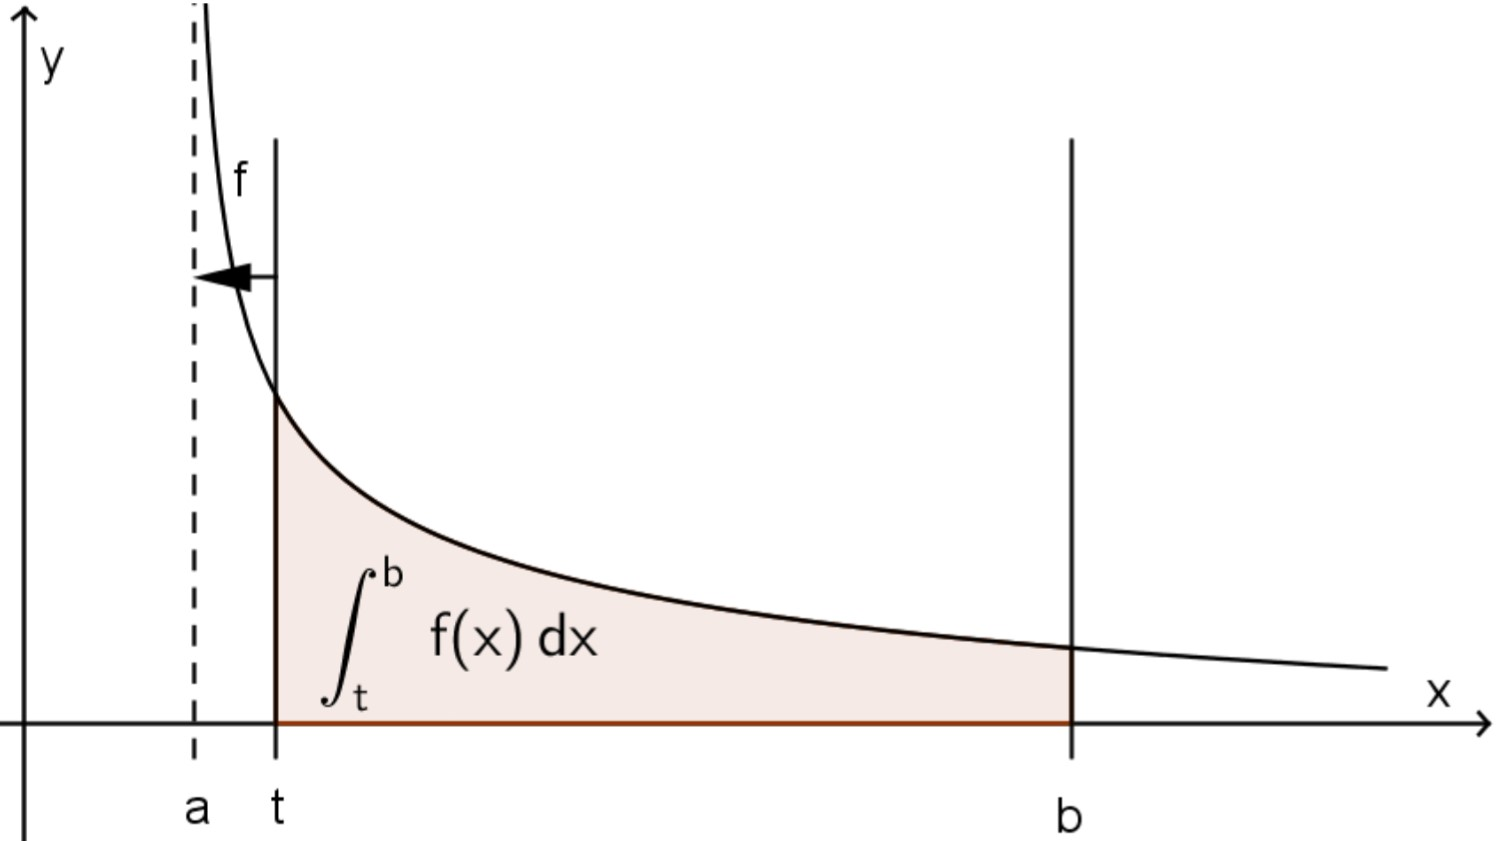
\includegraphics[scale=0.18]{uneigentlicher-integral-2}
        \end{center}
    \end{multicols}
\end{definition}

\textbf{Bemerkung:} Falls die Funktion auf der rechten Seite gegen unendlich strebt, dann lässt sich die obige Definition entsprechend anpassen:
\[\int \limits_{a}^{b} f(x) \diff{x} = \lim_{t \to b} \int \limits_{a}^{t} f(x) \diff{x}\]

\textbf{Beispiele:}
\begin{itemize}
    \item $\displaystyle \int \limits_{0}^{1} \frac{1}{\sqrt{x}} \diff{x} = \lim_{t \to 0} \int \limits_{t}^{1} \frac{1}{\sqrt {x}} \diff{x} = \lim_{t \to 0} \int \limits_{t}^{1} x^{-0.5} \diff{x} = \lim_{t \to 0} \left[ 2x^{0.5} \right]_{t}^{1} = 2 \sqrt{1} - 2 \sqrt {t} \xrightarrow[t \to 0]{} 2$
    \item $\displaystyle \int \limits_{0}^{1} \frac{1}{x} \diff{x} = \lim_{t \to 0} \int \limits_{t}^{1} \frac{1}{x} \diff{x} = \lim_{t \to 0} \left[ \ln(|x|) \right]_{t}^{1} = \lim_{t \to 0} \ln(1) - \ln(t) \xrightarrow[t \to 0]{} 0 - (-\infty) = \infty$ \\
    (Das Integral existiert also nicht)
\end{itemize}

    \section{Einführung in die Differentialgleichungen}\label{sec:einfuhrung-in-die-differentialgleichungen}

\subsection{Definition}\label{subsec:definition}

Differentialgleichungen sind eine spezielle Art von \emph{Funktionalgleichungen}: Diese sind Gleichungen, deren Lösungen nicht Zahlen, sondern Funktionen sind.

\begin{definition}{Definition}
    Eine \emph{Differentialgleichung} ist eine Funktionalgleichung, in der (unter anderem) die gesuchte Funktion, ihre Ableitung und ihre Variablen vorkommen.
    Wichtig zu bemerken ist, dass eine Differentialgleichung eine Beziehung zwischen einer Grösse und ihrer Veränderung ausdrückt.
\end{definition}

\textbf{Beispiele:}
\begin{itemize}
    \item $y' = 0$ \\ Eine Lösung: $y = 17$ \\ Allgemeine Lösung: $y = C$ \\ Kontrolle: $y' = (C)' = 0$
    \item $y' = y$ \\ Eine Lösung: $y = e^x$ \\ Allgemeine Lösung: $y = C \cdot e^x$ \\ Kontrolle: $y' = C \cdot e^x = y$
    \item $y' = 7y$ \\ Eine Lösung: $y = e^{7x}$ \\ Allgemeine Lösung: $y = C \cdot e^{7x}$ \\ Kontrolle: $y' = C \cdot 7e^{7x}$, $7y = 7Ce^{7x}$
    \item Beim radioaktiven Zerfall lässt sich die Menge der noch vorhandener Substanz durch folgende Differentialgleichung beschreiben: $y' = -\alpha \cdot y$ ($\alpha$ bezeichnet die sogenannte Proportionalitätskonstante). \\ Eine Lösung: $y = e^{-\alpha t}$ \\ Allgemeine Lösung: $y = C \cdot e^{-\alpha t}$ \\ Kontrolle: $y' = (C \cdot e^{-\alpha t})' = C \cdot (-\alpha) \cdot e^{-\alpha t}$, $-\alpha \cdot y = -\alpha \cdot C \cdot e^{-\alpha t}$
\end{itemize}

\textbf{Bedeutung der Konstanten $C$}

Im obigen Beispiel $t = 0$ einsetzen ergibt $y(0) = C$, d.h. $C$ ist die Menge der Substanz zum Zeitpunkt $t = 0$.
Ist diese Menge $m_0$ vorgegeben, so kommt nur noch eine Lösung infrage: $y(t) = m_0 \cdot e^{-\alpha t}$

Diese Lösung heisst \emph{partikuläre Lösung zur Anfangsbedingung $y(0) = m_0$}, im Gegensatz zur \emph{allgemeinen Lösung}, bei welcher nicht festgelegt ist, welchen Wert die Konstante C annehmen muss.

\begin{definition}{Weitere Definitionen}
    \begin{itemize}
        \item Die \emph{Ordnung} einer Differentialgleichung bezeichnet die Ordnung der höchsten vorkommenden Ableitung.
        \item Die \emph{allgemeine Lösung} einer Differentialgleichung $n$-ter Ordnung ist nie eindeutig bestimmt, sondern enthält noch $n$ voneinander unabhängige Parameter.
        \item Die \emph{partikuläre Lösung} wird durch zusätzliche Bedingungen festgelegt:
        \begin{itemize}
            \item \emph{Anfangsbedingungen:} vorgegebene Werte für $y(x_0)$, $y'(x_0)$, \dots, $y^{(n-1)}(x_0)$
            \item \emph{Randbedingungen:} vorgegebene Werte für $y(x_1)$, $y(x_2)$, \dots, $y(x_n)$
        \end{itemize}
    \end{itemize}
\end{definition}

\newpage

\subsection{Gewöhnliche Differentialgleichungen 1. Ordnung}\label{subsec:gewoehnliche-differentialgleichungen-1.-ordnung}

Eine Differentialgleichung heisst \emph{gewöhnlich}, wenn die gesuchte Funktion eine Funktion von \emph{einer} Variable ist.
Hat die gesuchte Funktion jedoch mehrere Variablen, dann nennt man das eine \emph{partielle} Differentialgleichung.

\begin{definition}{Allgemeine Differentialgleichung 1. Ordnung}
    \emph{Allgemeine Differentialgleichungen 1. Ordnung} haben die Form \[y' = F(x,y)\] wobei $F(x,y)$ ein Ausdruck ist, in dem $x$ und $y$ vorkommen.
\end{definition}

Die \emph{allgemeine} Lösung einer solchen Differentialgleichung enthält einen Parameter, und für jeden Wert dieses Parameters bekommen wir eine Lösung.
Diese Lösungen sind Funktionen und können als Graphen im Koordinatensystem dargestellt werden.

Wir möchten nun Informationen über die Menge dieser Graphen gewinnen.
Dazu fixieren wir einen Punkt $(x_0, y_0)$.
Wenn eine Funktion $f$ eine Lösung der obenstehenden Differentialgleichung ist, dann gilt für jeden Punkt $(x_0, y_0)$ auf ihrem Graph: \[f'(x_0) = F(x_0, y_0)\]
Mit anderen Worten: Falls eine Lösungskurve durch $(x_0, y_0)$ geht, dann hat sie in diesem Punkt die Steigung $F(x_0, y_0)$.
Wir können also diese Steigung ausrechnen, ohne die Lösungsfunktion $f$ zu kennen!

\textbf{Beispiel:} $y' = x-y+1$

Tabelle für $y^{\prime}$ :
\begin{tabular}{|c|c|c|c|c|c|c|c|}
    \hline
    $f'(x_0, y_0)$ & $x_0=-3$ & $x_0=-2$ & $x_0=-1$ & $x_0=0$ & $x_0=1$ & $x_0=2$ & $x_0=3$ \\
    \hline
    $y_0=2$        & -4       & -3       & -2       & -1      & 0       & 1       & 2       \\
    \hline
    $y_0=1$        & -3       & -2       & -1       & 0       & 1       & 2       & 3       \\
    \hline
    $y_0=0$        & -2       & -1       & 0        & 1       & 2       & 3       & 4       \\
    \hline
    $y_0=-1$       & -1       & 0        & 1        & 2       & 3       & 4       & 5       \\
    \hline
    $y_0=-2$       & 0        & 1        & 2        & 3       & 4       & 5       & 6       \\
    \hline
\end{tabular}

\textbf{Skizze des Richtungsfeldes}
\begin{center}
    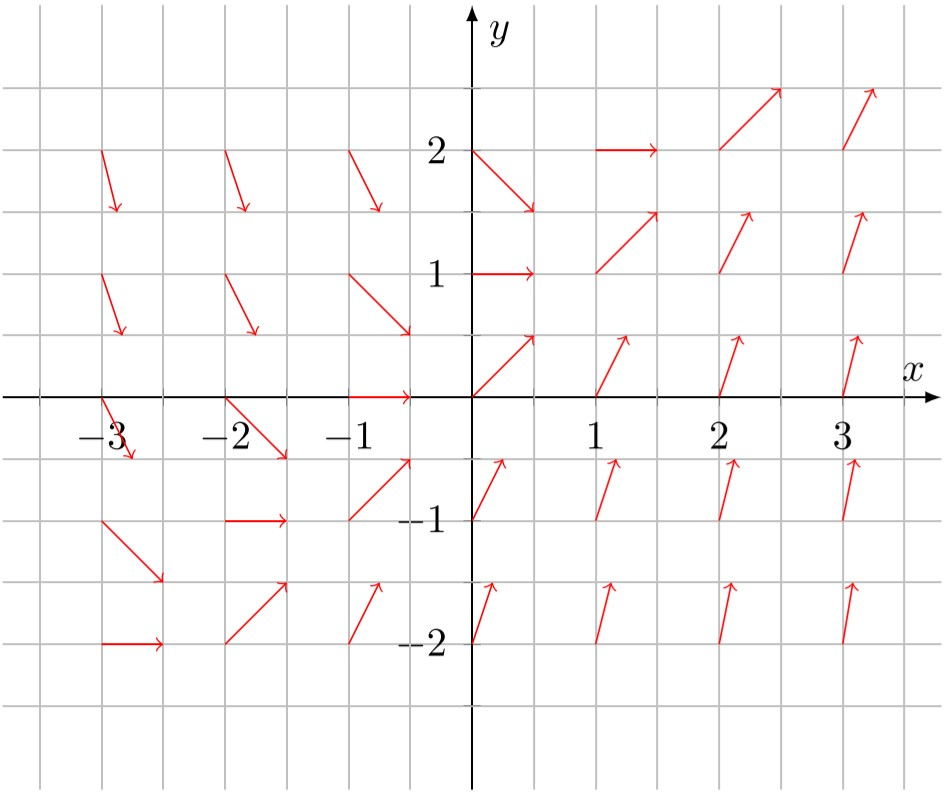
\includegraphics[scale=0.25]{skizze-richtungsfeld}
\end{center}

\textbf{Numerischer Lösungsansatz: Euler-Schritte}

Grund-Idee: An einem Punkt $(x_0,y_0)$ starten und dann der aktuellen Tangente folgen.
\begin{center}
    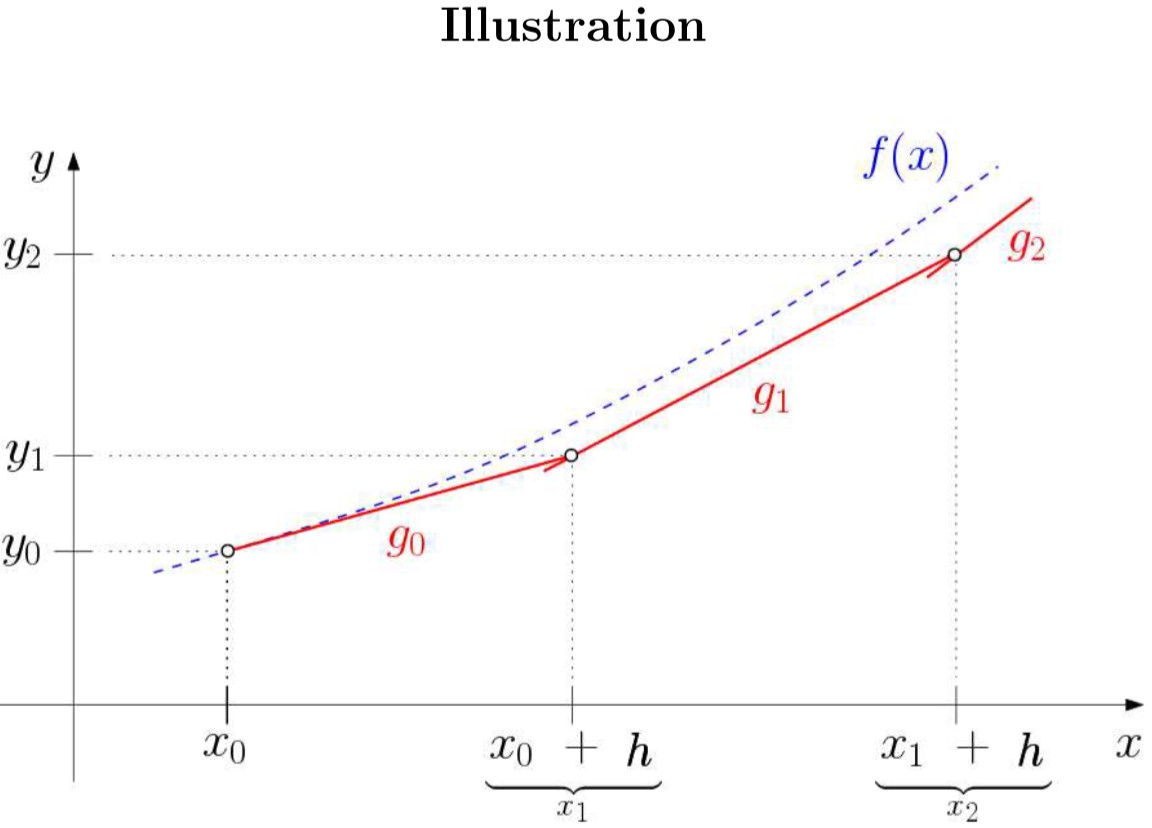
\includegraphics[scale=0.20]{skizze-euler-schritte}
\end{center}

\textbf{Beispiel:} $y' = \underbrace{x+y}_{F(x, y)}$, $x_0 = 0$, $y_0 = 1$, $h = 1$
\begin{center}
    \begin{tabular}{|l|l|l|}
        \hline
        Steigung Gerade &
        Berechnung &
        Beispiel \\
        \hline
        $g_0: m_0=F(x_0, y_0) = x_0 + y_0$   & $x_1 = x_0 + h$                   & $= 0 + 1 = 1$                \\
        & $y_1 = y_0 + h \cdot F(x_0, y_0)$ & $= 1 + 1 \cdot (0 + 1) = 2$  \\
        \hline
        $g_1: m_1 = F(x_1, y_1) = x_1 + y_1$ & $x_2 = x_1 + h$                   & $= 1 + 1 = 2$                \\
        & $y_2 = y_1 + h \cdot F(x_1, y_1)$ & $= 2 + 1 \cdot (1 + 2) = 5$  \\
        \hline
        $g_2: m_2=F(x_2, y_2) = x_2 + y_2$   & $x_3 = x_2 + h$                   & $= 2 + 1 = 3$                \\
        & $y_3 = y_2 + h \cdot F(x_2, y_2)$ & $= 5 + 1 \cdot (2 + 5) = 12$ \\
        \hline
    \end{tabular}
\end{center}

Die obigen Operationen nennt man \emph{Euler-Schritte}.
Der Abstand $h$ zwischen den betrachteten $x$-Werten heisst $Schrittweite$.
Wählt man die Schrittweite sehr, sehr klein, so lassen sich für viele Differentialgleichungen die gewünschten Funktionswerte relativ genau bestimmen.

\subsection{Separierbare Differentialgleichungen}\label{subsec:separierbare-differentialgleichungen}

\begin{definition}{Definition Separierbarkeit}
    Eine Differentialgleichung 1.\ Ordnung heisst \emph{separierbar}, wenn sie sich in der folgenden Form schreiben lässt: \[y' = f(x) \cdot g(y)\]
\end{definition}

\textbf{Beispiele:}
\begin{itemize}
    \item $y' = (x^2 + \sin(x)) \cdot (e^y - y + 7)$ ist eine separierbare Differentialgleichung.
    \item $y' = x - y + 1$ ist \emph{nicht} separierbar.
\end{itemize}

\begin{subbox}{Rezept für die Lösung von separierbaren Differentialgleichungen}
    \begin{enumerate}
        \item $y' = \frac{\diff{y}}{\diff{x}} = f(x) \cdot g(x)$
        \item Trennung der Variablen: $\frac{\diff{y}}{g(y)} = f(x) \cdot \diff{x}$
        \item Integration auf beiden Seiten der Gleichung (falls möglich!) \[\int \frac{\diff{y}}{g(y)} = \int f(x) \diff{x}\]
        \item Auflösen nach $y$ (falls möglich!)
    \end{enumerate}
\end{subbox}

\begin{multicols}{2}
    \textbf{Beispiel 1:} $y' = k \cdot y$
    \begin{enumerate}
        \item $y' = \frac{\diff{y}}{\diff{x}} = k \cdot y$
        \item $\frac{\diff{y}}{y} = k \cdot \diff{x}$
        \item $\int \frac{\diff{y}}{y} = \int k \diff{x} \Rightarrow \ln |y| = k \cdot x + C$
        \item $|y| = e^{kx + C} = e^C \cdot e^{kx} \Rightarrow y = \pm e^C \cdot e^{kx} = \tilde{C} e^{kx}$
    \end{enumerate}

    \textbf{Beispiel 2:} $y' \cdot y^2 = \sin(x)$
    \begin{enumerate}
        \item $y' = \frac{\diff{y}}{\diff{x}} = \frac{\sin(x)}{y^2}$
        \item $y^2 \cdot \diff{y} = \sin(x) \cdot \diff{x}$
        \item $\int y^2 \diff{y} = \int \sin(x) \diff{x} \Rightarrow \frac{1}{3} y^3 = -\cos(x) + C$
        \item $y = (-3\cos(x) + 3C)^{1/3}$
    \end{enumerate}
\end{multicols}

\vspace{-\baselineskip}
\hrulefill

\begin{multicols}{2}
    \textbf{Beispiel 3:} $x + y \cdot y' = 0$ mit Anfangsbedingung $y(3) = -4$
    \begin{enumerate}
        \item $y' = \frac{\diff{y}}{\diff{x}} = - \frac{x}{y}$
        \item $y \cdot \diff{y} = -x \diff{x}$
        \item $\int y \diff{y} = - \int x \diff{x} \Rightarrow \frac{y^2}{2} = - \frac{x^2}{2} + C$
        \item $x^2 + y^2 = C_2$ (Kreisgleichung) \\
        $\Rightarrow y = \pm \sqrt {C_2 - x^2}$ (keine Funktion)
    \end{enumerate}
    \textbf{Einbezug der Anfangsbedingung $y(3) = -4$:}

    Einsetzen von $x = 3, y = -4$ in obige Gleichung liefert:

    $-4 = - \sqrt {C_2 - 9} \Rightarrow C_2 - 9 = 16 \Rightarrow C_2 = 25$

    Lösung: $y = - \sqrt {25 - x^2}$
\end{multicols}

\begin{comment}
    \begin{definition}{Autonome Differentialgleichungen}
        Eine Differentialgleichung heisst \emph{autonom}, wenn sie sich in der folgenden Form darstellen lässt: \[y' = f(y)\]
    \end{definition}

    \textbf{Beispiele}
    \begin{center}
        \begin{tabular}{|l|l|}
            \hline
            \multicolumn{1}{|c|}{ Gleichung }            & Autonom?                                                      \\
            \hline
            $y' = y^2 + 6$                               & Ja $\Rightarrow f(y) = y^2 + 6$                               \\
            \hline
            $y' = x + y$                                 & Nein                                                          \\
            \hline
            $y' = \frac{y}{x}$                           & Nein                                                          \\
            \hline
            $y' = y^2 \cdot \sqrt{1 - \sin(y)} - \ln(y)$ & Ja $\Rightarrow f(y) = y^2 \cdot \sqrt{1 - \sin(y)} - \ln(y)$ \\
            \hline
        \end{tabular}
    \end{center}

    \textbf{Lösungsmethode:} Diese Differentialgleichungen sind separierbar!
\end{comment}

\subsection{Lineare Differentialgleichungen 1. Ordnung}\label{subsec:lineare-differentialgleichungen-1.-ordnung}

\begin{definition}{Lineare Differentialgleichungen}
    Eine Differentialgleichung 1.\ Ordnung heisst \emph{linear}, wenn sie die Form \[y' + f(x) \cdot y = g(x)\] hat, wobei $f$ und $g$ Funktionen von $x$ sind.
    Die Funktion $g(x)$ wird als \emph{Störglied} oder \emph{Störfunktion} bezeichnet.
\end{definition}

\textbf{Bemerkung:} Die Bezeichnung \emph{linear} bezieht sich einzig darauf, dass $y$ und $y'$ nur in der ersten Potenz vorkommen.
Die Funktionen $f(x)$ und $g(x)$ hingegen brauchen keineswegs linear zu sein.

\begin{center}
    \begin{tabular}{|c|c|c|}
        \hline
        Differentialgleichung                                    & $f(x)$        & $g(x)$                          \\
        \hline
        $y' = xy$                                                & $-x$          & $0$                             \\
        \hline
        $xy' + 2y = e^x$                                         & $\frac{2}{x}$ & $\frac{e^x}{x}$                 \\
        \hline
        $y' = (\tan(x)) \cdot y + 2 \cdot \sin(x) \cdot \cos(x)$ & $-\tan(x)$    & $2 \cdot \sin(x) \cdot \cos(x)$ \\
        \hline
    \end{tabular}
\end{center}

\begin{definition}{Homogene DGL}
    Eine lineare Differentialgleichung heisst \emph{homogen}, wenn das Störglied $g(x) = 0$ ist.
    Ansonsten nennt man sie \emph{inhomogen}.

    Betrachtet man eine \emph{inhomogene} lineare Differentialgleichung $y' + f(x) \cdot y = g(x)$, dann bezeichnet man die \emph{zugehörige homogene Differentialgleichung} die Gleichung $y_0' + f(x) \cdot y_0 = 0$.
\end{definition}

Grundsätzlich sind homogene Differentialgleichungen leichter zu lösen als inhomogene.
Unser Lösungsverfahren für lineare Differentialgleichungen besteht deshalb aus zwei Schritten:
\begin{enumerate}
    \item Lösung der zugehörigen Differentialgleichung bestimmen.
    \item Ursprüngliche Differentialgleichung durch \emph{Variation der Konstanten} lösen.
\end{enumerate}

\begin{subbox}{Rezept: Variation der Konstanten}
    \begin{enumerate}
        \item Vergleich der \emph{gegebenen} Differentialgleichung mit der \emph{allgemeinen} Form $y' + f(x) \cdot y = g(x)$ und Bestimmung von $f(x)$ und $g(x)$.
        \item Bestimmung der Stammfunktion $F(X)$ von $f(x)$.
        \item Einsetzen in die Formel $y_0 = C \cdot e^{-F(x)}$ liefert die Lösung der zugehörigen \emph{homogenen} Differentialgleichung.
        \item Ein Einsetzen von $C$ durch eine noch zu bestimmende Funktion $K(x)$ führt zum folgenden Ansatz für die allgemeine Lösung: \[y = K(x) \cdot e^{-F(x)}\]
        \item Die Funktion $K(x)$ lässt sich durch die folgende Formel berechnen: \[K(x) = \int g(x) \cdot e^{F(x)} \diff{x} \quad\quad\quad \text{(Integrationskonstante nicht vergessen!)}\]
        \item Einsetzen von $K(x)$ in den Ansatz aus Schritt 4 ergibt die \emph{allgemeine Lösung}.
    \end{enumerate}
\end{subbox}

\textbf{Beispiel:} $y' + \frac{y}{x} = \cos(x)$
\begin{enumerate}
    \item $f(x) = \frac{1}{x}$, $g(x) = \cos(x)$
    \item $F(x) = \ln(x)$
    \item $y_0 = \frac{C}{x}$
    \item Ansatz: $y = \frac{K(x)}{x}$
    \item $K(x) = \int g(x) \cdot e^{F(x)} \diff{x} = \int \cos(x) \cdot x \diff{x} = x \cdot \sin(x) + \cos(x) + C_2$
    \item $K(x)$ in den Ansatz von Schritt 4 einsetzen: $y = \frac{x \cdot \sin(x) + \cos(x) + C_2}{x}$
\end{enumerate}

    \section{Anwendung der Integralrechnung}\label{sec:anwendung-der-integralrechnung}

\textbf{Repetition:} Das \emph{bestimmte Integral} einer Funktion $f$ ist wie folgt definiert: \[\int_{a}^{b} f(x) \diff{x} = \lim_{n \rightarrow \infty} \sum_{k=1}^{n} f(x_K) \Delta x\]

\subsection{Mittelwert}\label{subsec:mittelwert}

\begin{center}
    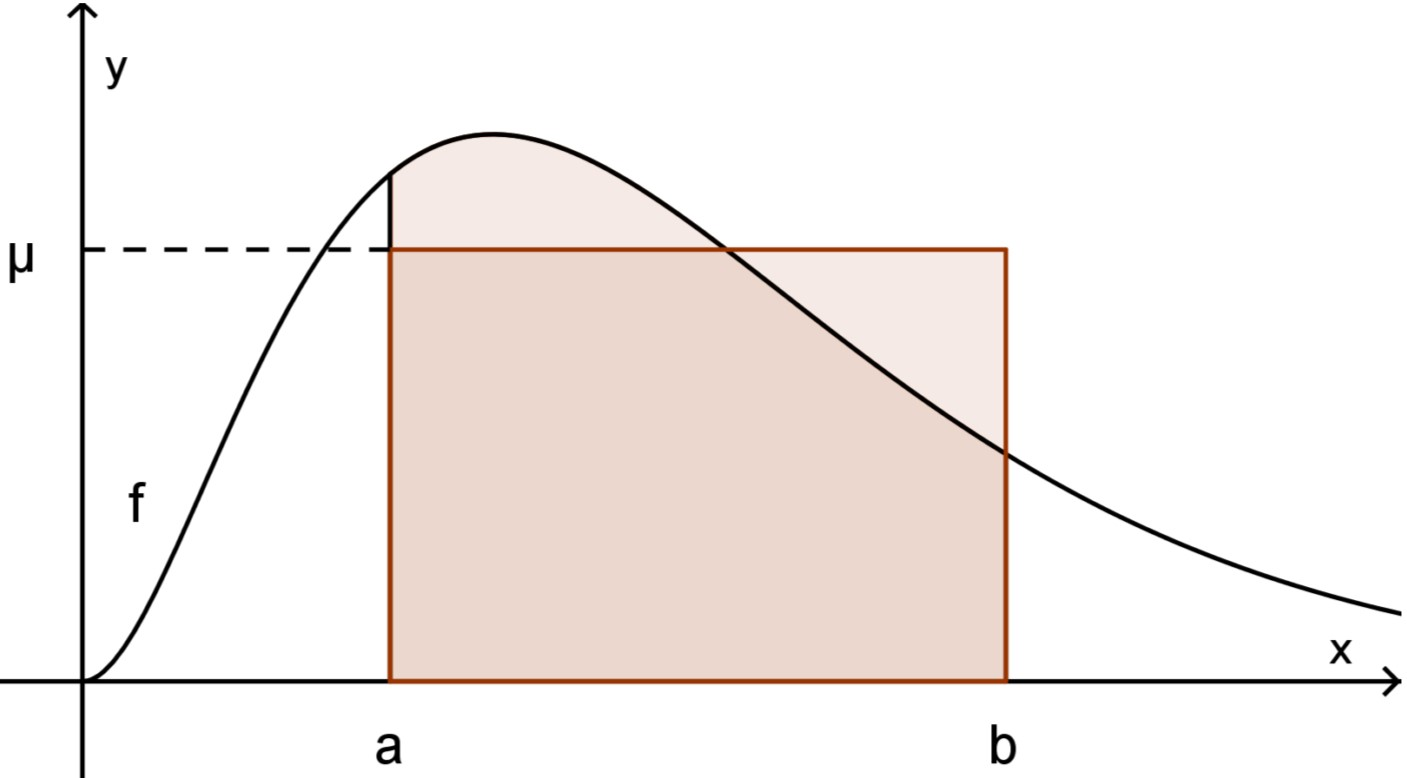
\includegraphics[scale=0.15]{mittelwert}
\end{center}

\begin{definition}{Mittelwert}
    Gegeben ist eine Funktion $f$ mit $f(x) \leq 0$ für alle $x \in [a,b]$.
    Unter dem \emph{Mittelwert} $\mu$ von $f$ versteht man die Höhe jenes Rechtecks,
    \begin{itemize}
        \item das eine Grundlinie der Länge $b - a$ hat, und
        \item dessen Flächeninhalt der Fläche unter der Kurve, resp. $\int_{a}^{b} f(x) \diff{x}$, entspricht.
    \end{itemize}
    Daraus folgt: \[\mu = \frac{1}{b - a} \cdot \int_{a}^{b} f(x) \diff{x}\]
\end{definition}

\textbf{Beispiel:} Berechnen Sie den Mittelwert von $f(x) = x^2 + 2$ auf dem Intervall $[2,4]$.
\begin{align*}
    \mu &= \frac{1}{4 - 2} \cdot \int_{2}^{4} (x^2 + 2) \diff{x} = \frac{1}{2} \cdot \left( \int_{2}^{4} x^2 \diff{x} + \int_{2}^{4} 2 \diff{x} \right) = \frac{1}{2} \cdot \left( \left[ \frac{x^3}{3} \right]_{2}^{4} + \left[ 2x \right]_{2}^4 \right) \\
    &= \frac{1}{2} \cdot \left( \frac{4^3}{3} - \frac{2^3}{3} + (8 - 4) \right) = \frac{34}{3}
\end{align*}

\subsection{Volumen eines Rotationskörpers}\label{subsec:volumen-eines-rotationskorpers}

\begin{definition}{Volumen eines Rotationskörpers (Drehung um $x$-Achse)}
    Gegeben ist eine Funktion $f$ mit $f(x) \leq 0$ für alle $x \in [a,b]$.
    Dreht man das Flächenstück um die $x$-Achse, so entsteht ein \emph{Rotationskörper} mit dem folgenden Volumen: \[V = \pi \cdot \int_{a}^{b} (f(x))^2 \diff{x}\]
\end{definition}

\begin{center}
    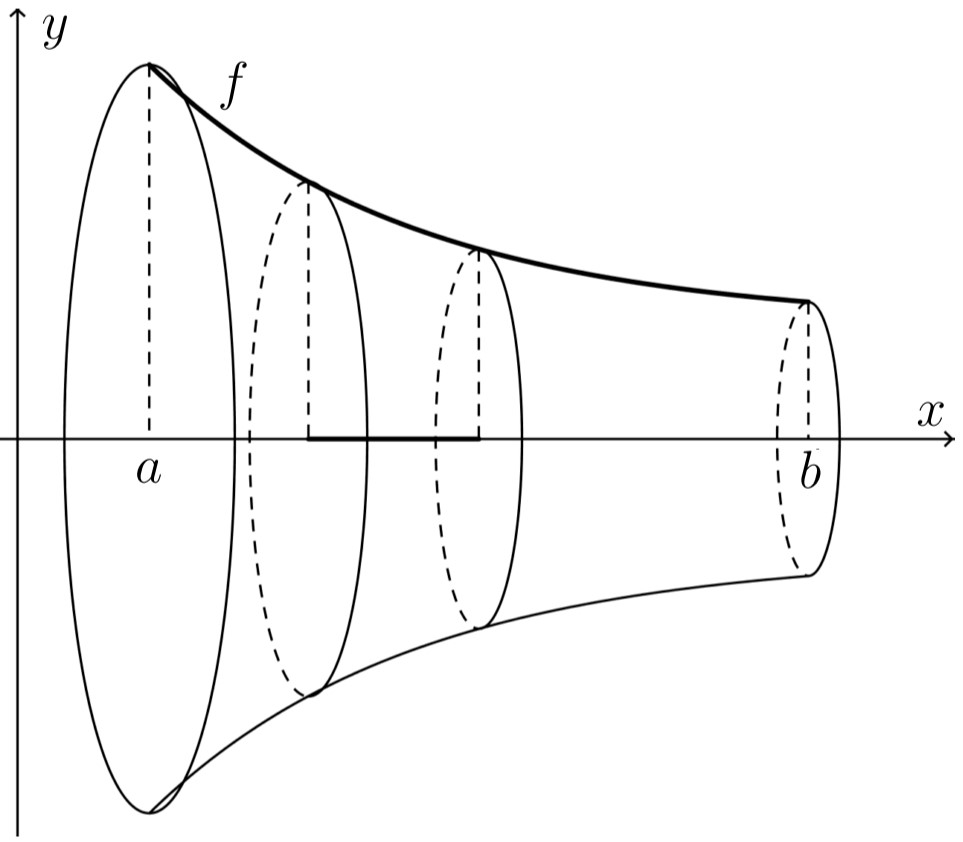
\includegraphics[scale=0.25]{volumen-rotationskoerper}
\end{center}

\textbf{Beispiel:} $f(x) = x^2 + 1$, $a = -1$, $b = 1$.
Berechnen Sie das Volumen des entsprechenden Rotationskörpers.
\begin{align*}
    V &= \pi \int_{-1}^{1} (x^2 + 1)^2 \diff{x} = \pi \int_{-1}^{1} x^4 + 2 x^2 + 1 \diff{x} = \pi \left( \int_{-1}^{1} x^4 \diff{x} + 2 \int_{-1}^{1} x^2 \diff{x} + \int_{-1}^{1} 1 \diff{x} \right) \\
    &= \pi \left( \left[ \frac{x^5}{5} \right]_{-1}^{1} + 2 \left[ \frac{x^3}{3} \right]_{-1}^{1} + [x]_{-1}^{1} \right) = \pi \left( \frac{1}{5} - \left( -\frac{1}{5} \right) + 2 \cdot \left( \frac{1}{3} - \left( -\frac{1}{3} \right) \right) + 1 - (-1) \right) = \frac{56}{15} \pi
\end{align*}

\begin{definition}{Volumen eines Rotationskörpers (Drehung um $y$-Achse)}
    Gegeben ist eine Funktion $y = f(x)$ mit $x \leq 0$ für alle $y \in [c, d]$.
    Dreht man das Flächenstück, das zwischen dem Graphen von $f$, der $y$-Achse und den beiden Grenzen $y = c$ und $y = d$ liegt, \textbf{um die $y$-Achse}, so entsteht ein Rotationskörper mit den folgenden Volumen: \[V = \pi \cdot \int_{c}^{d} (g(y))^2 \diff{y}\] wobei $g(y)$ die nach $x$ aufgelöste Funktionsgleichung ist.
\end{definition}

\begin{center}
    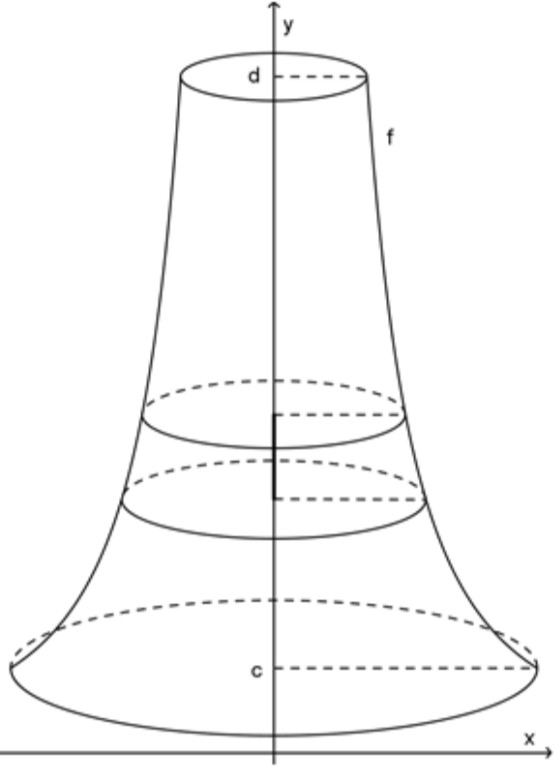
\includegraphics[scale=0.25]{volumen-rotationskoerper-y-achse}
\end{center}

\textbf{Beispiel:} Das Kurvenstück $y = \sqrt {x}$ wird im Intervall $0 \geq y \geq 5$ um die $y$-Achse rotiert.
Wie gross ist das Volumen des entsprechenden Rotationskörpers?

$y = \sqrt {x}$ \\
Umkehrfunktion: $y^2 = x \Rightarrow g(y) = y^2$

$\Rightarrow V = \pi \int_{0}^{5} (y^2)^2 \diff{y} = \pi \int_{0}^{5} y^4 \diff{y} = \pi \cdot \left[ \frac{y^5}{5} \right]_{0}^{5} = \pi \cdot \frac{5^5}{5} = 625 \pi$

\subsection{Bogenlänge einer ebenen Kurve}\label{subsec:bogenlange-einer-ebenen-kurve}

\begin{definition}{Bogenlänge einer ebenen Kurve}
    Wir betrachten eine Funktion $y = f(x)$ über einem Intervall $[a,b]$.
    Die Bogenlänge dieser Kurve beträgt \[s = \int_{a}^{b} \sqrt {1 + (y')^2} \diff{x}\]
\end{definition}

\begin{center}
    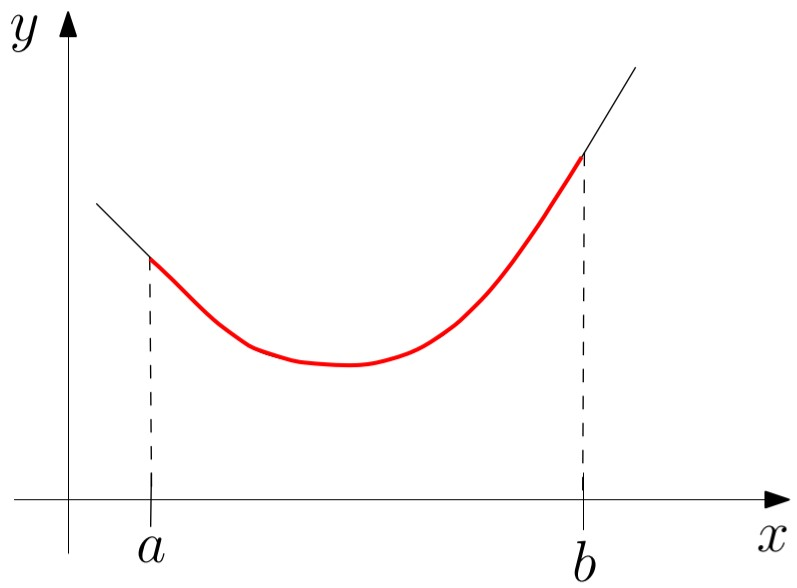
\includegraphics[scale=0.25]{bogenlaenge}
\end{center}

\newpage

\subsection{Mantelfläche eines Rotationskörpers}\label{subsec:mantelflache-eines-rotationskorpers}

\begin{definition}{Mantelfläche eines Rotationskörpers}
    Die \emph{Mantelfläche} bezeichnet die Oberfläche eines Körpers ohne seinen Deckel und Boden.
    Wir betrachten eine Funktion $y = f(x)$ mit $f(x) \leq 0$ für alle $x \in [a,b]$.
    Dreht man das Flächenstück, das im Intervall $[a,b]$ zwischen dem Graphen von $f$ und der $x$-Achse liegt, um die $x$-Achse, so entsteht ein Rotationskörper mit der folgenden Mantelfläche: \[M = 2 \pi \cdot \int_{a}^{b} y \cdot \sqrt {1 + (y')^2} \diff{x}\]
\end{definition}

\textbf{Beispiel:}

Das Kurvenstück $y = \sqrt{x}$ wird im Intervall $0 \geq x \geq 2$ um die $x$-Achse rotiert.
Berechnen Sie die Mantelfläche des entstehenden \emph{Paraboloids}.

$y = \sqrt{x} = x^{1/2}$, $y' = \frac{1}{2} x^{-1/2)}$, $1 + (y')^2 = 1 + \frac{1}{4x}$

$M = 2 \pi \int_{0}^{2} \sqrt{x} \cdot \sqrt {1 + \frac{1}{4x}} \diff{x} = 2 \pi \int_{0}^{2} \sqrt {x + \frac{1}{4}} \diff{x} = 2 \pi \cdot \left[ \frac{2}{3} \left( x + \frac{1}{4} \right)^{3/2} \right]_{0}^{2} = \frac{13 \pi}{3} \approx 13.61$

\subsection{Schwerpunkt}\label{subsec:schwerpunkt}

\begin{definition}{Bedeutung Schwerpunkt (Physik)}
    Ein fester Körper verhält sich häufig so, als wäre seine gesamte Masse in seinem \emph{Schwerpunkt} vereinigt.
    Diese ist sozusagen das gewichtete Mittel aller Massenpunkte.
\end{definition}

\begin{definition}{Schwerpunkt einer Fläche zwischen zwei Kurven}
    \begin{multicols}{2}
        Der Schwerpunkt des Flächenstücks, das im Intervall $[a,b]$ zwischen den Graphen von $f_o(x)$ und $f_u(x)$ liegt, hat die Koordinaten:
        \begin{align*}
            &x_s = \frac{1}{A} \int_{a}^{b} x \cdot (f_o(x) - f_u(x)) \diff{x} \\
            &y_s = \frac{1}{2A} \int_{a}^{b} (f_o^2(x) - f_u^2(x)) \diff{x}
        \end{align*}
        \begin{center}
            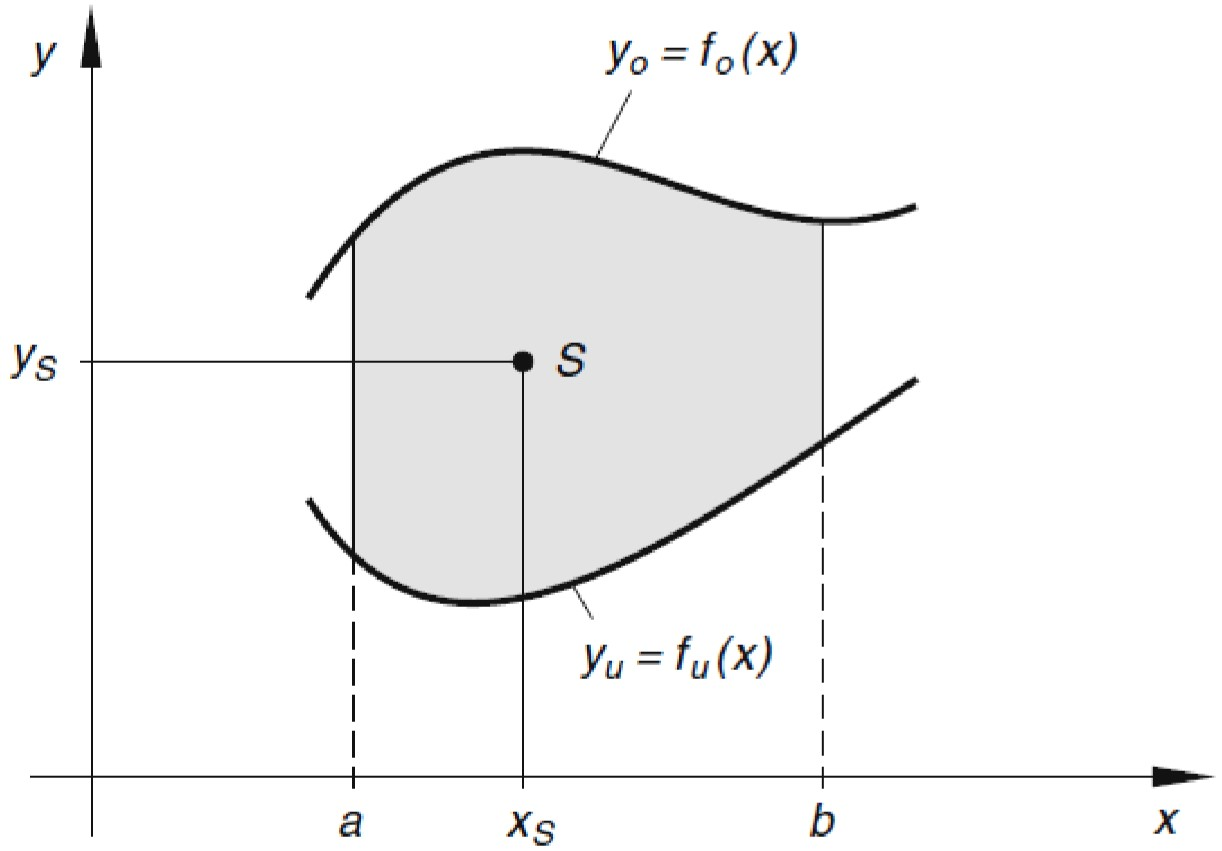
\includegraphics[scale=0.25]{schwerpunkt-flaeche}
        \end{center}
    \end{multicols}
\end{definition}

\begin{definition}{Schwerpunkt eines Rotationskörpers}
    \begin{multicols}{2}
        Wir betrachten eine Funktion $y = f(x)$ mit $f(x) \leq 0$ für alle $x \in [a,b]$.
        Dreht man das Flächenstück, das im Intervall $[a,b]$ zwischen dem Graphen von $f$ und der $x$-Achse liegt, um die $x$-Achse, so entsteht ein Rotationskörper.
        Sein Schwerpunkt hat folgende Koordinaten:
        \[x_s = \frac{\pi}{V} \int_{a}^{b} x \cdot f^2(x) \diff{x} \quad\quad y_s = 0 \quad\quad z_s = 0\]
        \begin{center}
            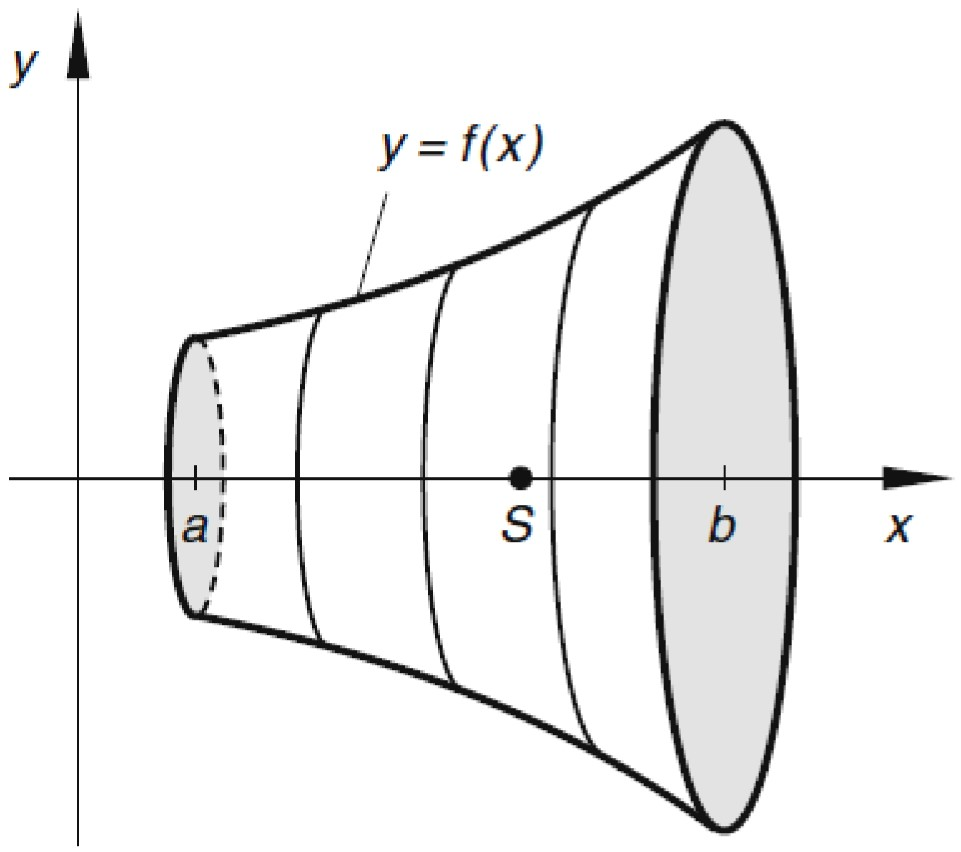
\includegraphics[scale=0.25]{schwerpunkt-koerper}
        \end{center}
    \end{multicols}
\end{definition}

    \section{Approximation durch Polynomfunktionen (Taylor-Reihen)}\label{sec:approximation-durch-polynomfunktionen}

\subsection{Taylor-Reihe}\label{subsec:taylor-reihe}

\begin{definition}{Taylor-Reihe}
    Wir betrachten eine Funktion $f$ und eine Stelle $x_0$ in ihrem Definitionsbereich.
    \begin{itemize}
        \item Das \emph{Taylor-Polynom vom Grad $n$ von $f$ um $x_0$} bezeichnet das Polynom \[p_n = \sum_{k=0}^{n} \frac{f^{(k)} (x_0)}{k!} \cdot (x - x_0)^k\]
        \item Die \emph{Taylor-Reihe} von $f$ um $x_0$ bezeichnet die unendliche Reihe \[t_f(x) = \sum_{k=0}^{\infty} \frac{f^{(k)} (x_0)}{k!} \cdot (x - x_0)^k\]
    \end{itemize}
\end{definition}

\textbf{Beispiel 1:} Bestimmen Sie die Taylor-Reihe von $f(x) = e^x$ um $x_0 = 0$.

$f(x_0) = 1$, $f'(x_0) = e^{x_0} = 1$, $f''(x_0) = e^{x_0} = 1$

Allgemein: $f^{(k)}(x_0) = e^{x_0} = 1$

$\Rightarrow t_f(x) = \sum_{k=0}^{\infty} \frac{1}{k!} x^k$

\textbf{Beispiel 2:} Bestimmen Sie die Taylor-Reihe von $f(x) = e^{-x^2}$ um $x_0 = 0$

Einsetzen in die Taylor-Reihe von $e^z \left(= 1 + z + \frac{z^2}{2!} + \frac{z^3}{3!} + \dots \right)$: \[t_f(x) = 1 - x^2 + \frac{x^4}{2!} - \frac{x^6}{3!} + \dots = \sum_{k=0}^{\infty} (-1)^k \cdot \frac{1}{k!} \cdot x^{2k}\]

\textbf{Beispiel 3:} Bestimmen Sie die Taylor-Reihe von $f(x) = \sin(x^3)$ um $x_0 = 0$

$\sin(z) = z - \frac{z^3}{3!} + \frac{z^5}{5!} - \dots$

Setzt man in dieser Reihe $z \coloneqq x^3$ ein, so bekommt man: \[t_f(x) = x^3 - \frac{x^9}{3!} + \frac{x^{15}}{5!} - \dots = \sum_{k=0}^{\infty} (-1)^k \cdot \frac{(x^3)^{2k+1}}{(2k + 1)!} = \sum_{k=0}^{\infty} \frac{(-1)^k \cdot x^{6k + 3}}{(2k + 1)!}\]

\subsection{Konvergenz}\label{subsec:konvergenz}

Die Taylor-Reihe hat die Eigenschaft, dass sie in der ``Nähe'' von $x_0$ die ursprüngliche Funktion sehr gut approximiert.
Bei sehr vielen Funktionen erreicht man sogar noch mehr: Bei ihnen ist der Funktionswert in einem bestimmten Intervall um $x_0$ herum exakt gleich dem Wert der Taylor-Reihe.
Es gilt also \[f(x) = \sum_{k=0}^{\infty} a_k = (x - x_0)^k\]
\textbf{Beispiele:}
\begin{itemize}
    \item $f(x) = \sin(x)$ mit $x_0 = 0$, im Intervall $\R$
    \item $f(x) = e^x$ mit $x_0 = 1$, im Intervall $\R$
    \item $f(x) = \frac{1}{x^2 + 1}$ mit $x_0 = 0$, im Intervall $(-1,1)$
\end{itemize}

In solchen Fällen sagt man, die Funktion $f(x)$ sei (im entscheidenden Intervall) \emph{durch ihre Taylor-Reihe $t_f(x)$ darstellbar}.

\textbf{Bemerkung:} Es gibt Kriterien, mit deren Hilfe man das entsprechende Intervall bestimmen kann, beispielsweise das sogenannte ``Quotientenkriterium'' und das sogenannte ``Wurzelkriterium''.

\begin{definition}{Konvergenz}
    Der \emph{Konvergenzbereich} bezeichnet all diejenigen $x$-Werte, bei denen $f(x)$ genau dem Wert der Taylor-Reihe entspricht.
\end{definition}

Für die obigen Beispiele bedeutet dies:
\begin{itemize}
    \item $f(x) = \sin(x)$ mit $x_0 = 0$ hat den Konvergenzbereich $\R$
    \item $f(x) = e^x$ mit $x_0 = 1$ hat den Konvergenzbereich $\R$
    \item Bei $f(x) = \frac{1}{x^2 + 1}$ mit $x_0 = 0$ gehört $(-1,1)$ zum Konvergenzbereich
\end{itemize}

\begin{definition}{Potenzreihe}
    \[P(x) = \sum_{k=0}^{\infty} a_k \cdot (x - x_0)^k\]
\end{definition}

\subsubsection{Konvergenzkriterien}

\begin{definition}{Quotientenkriterium}
    Für eine beliebige Potenzreihe $P(x) = \sum_{k=0}^{\infty} a_k (x - x_0)^k$ und $r \coloneqq \lim_{k \rightarrow \infty} \left| \frac{a_k}{a_{k+1}} \right|$ gilt:
    \begin{itemize}
        \item Alle $x$ mit $|x - x_0| < r$ gehören zum Konvergenzbereich
        \item Alle $x$ mit $|x - x_0| > r$ gehören \emph{nicht} zum Konvergenzbereich
    \end{itemize}
\end{definition}

\textbf{Konvention:} Falls der betrachtete Ausdruck gegen unendlich geht, so setzen wir $r$ auf ``$\infty$'', und alle $x \in \R$ gehören zum Konvergenzbereich.

\begin{definition}{Konvergenzradius}
    Das Quotientenkriterium besagt, dass \emph{alle} Werte, die sich innerhalb eines gewissen Maximal-Abstandes zu $x_0$ befinden, zum Konvergenzbereich gehören, während \emph{alle} Werte, die diesen Abstand überschreiten, nicht dazugehören.
    Es lässt sich zeigen, dass \emph{alle Potenzreihen} (auch diejenigen, für die das Quotientenkriterium nicht anwendbar ist) diese Eigenschaft haben!
    Es gilt also:

    Für \emph{jede} Potenzreihe $P(x) = \sum_{k=0}^{\infty} a_k (x - x_0)^k$ gibt es einen Abstand $r$, so dass
    \begin{itemize}
        \item alle $x \in (x_0 - r, x_0 + r)$ zum Konvergenzbereich gehören
        \item alle $x \in (-\infty, x_0 - r) \cup (x_0 + r, \infty)$ nicht zum Konvergenzbereich gehören
    \end{itemize}
\end{definition}

\subsection{Potenzreihe und Polynome}\label{subsec:potenzreihe-und-polynome}

Man kann zeigen, dass \emph{innerhalb} des Konvergenzbereiches Potenzreihen grundsätzlich wie Polynome behandelt werden können:
\begin{itemize}
    \item Die Ableitung von $P(x)$ lässt sich berechnen, indem man jedes Glied einzeln ableitet.
    \item Das Integral von $P(x)$ lässt sich berechnen, indem man jedes Glied einzeln integriert.
    \item Addition, Subtraktion und Multiplikation kann man ebenfalls wie bei gewöhnlichen Polynomen durchführen.
\end{itemize}

\textbf{Beispiel:} Wir betrachten die Potenzreihe $P(x) = \sum_{k=0}^{\infty} x^k = 1 + x + x^2 + x^3 + x^4 + \dots$
\begin{itemize}
    \item $P'(x) = 1 + 2x + 3x^2 + 4x^3 + \dots = \sum_{k=0}^{\infty} (k + 1)x^k$
    \item $\int P(x) \diff{x} = x + \frac{x^2}{2} + \frac{x^3}{3} + \frac{x^4}{4} + \dots = \sum_{k=0}^{\infty} \frac{1}{k + 1} \cdot x^{k + 1}$
    \item $P(x) + \sum_{k=0}^{\infty} kx^k = (1 + x + x^2 + x^3 + x^4 + \dots) + (x + 2x^2 + 3x^3 + \dots) = 1 + 2x + 3x^2 + 4x^3 + \dots = \sum_{k=0}^{\infty} (k + 1)x^k$
\end{itemize}

\subsubsection{Fehlerabschätzung bei der Taylor-Reihe}

Für viele Anwendungen ist es ``handlicher'', nur mit den ersten paar Summanden des Polynoms zu rechnen und die restlichen zu ignorieren.
Beachtlicherweise führt dies in ganz vielen Fällen nur zu kleinen, verkraftbaren Genauigkeitseinbussen!

\textbf{Eine Formel für Fehlerabschätzung:} Der Fehler, der bei der Beschränkung auf die Glieder von Grad $\leq n$ entsteht, bezeichnen wir mit $R_n$. \[R_n(x) = \sum_{k=0}^{\infty} \frac{f^{(k)}(x_0)}{k!} (x - x_0) - \sum_{k=0}^{n} \frac{f^{(k)}(x_0)}{k!} (x - x_0)^k\]

\subsection{Anwendungen der Taylor-Reihe}\label{subsec:anwendungen-der-taylor-reihe}

\subsubsection{Numerische Berechnungen von Funktionswerten}

\textbf{Beispiel:} Bestimmen Sie für den Wert $x=1.2$ zunächst mit dem Taschenrechner den auf 4 Kommastellen gerundeten Wert von $\sin(x)$.
Bestimmen Sie dann die \emph{Anzahl} benötigter Summanden der Taylor-Reihe, um den zuerst ermittelten Wert zu erhalten.

$\sin(1.2) = 0.9320$, Taylor-Reihe: $\sin(x) = x - \frac{x^3}{3!} + \frac{x^5}{5!} - \frac{x^7}{7!} + \dots$

$1.2 - \frac{1.2^3}{3!} + \frac{1.2^5}{5!} = 0.9327 \Rightarrow$ 3 Summanden sind zu wenig!

$1.2 - \frac{1.2^3}{3!} + \frac{1.2^5}{5!} + \frac{1.2^7}{7!} = 0.9320 \Rightarrow$ 4 Summanden reichen aus.

\subsubsection{Approximation für Integrale}

\textbf{Beispiel:} Bestimmen Sie einen Näherungswert für das Integral $\int_{0}^{1} e^{x^2} \diff{x}$, indem Sie mit einem Taylor-Polynom vom Grad 2 arbeiten.

Bestimmung des gesuchten Taylor-Polynoms: $e^x = 1 + x + \frac{x^2}{2!} + \frac{x^3}{3!} + \dots$

Also ist $e^{x^2} = 1 + x^2 + \frac{x^4}{2!} + \frac{x^6}{3!} + \dots$

Verwendet man das Taylor-Polynom vom Grad 2, so ergibt sich die Abschätzung $\displaystyle \int_{0}^{1} e^{x^2} \diff{x} \approx \int_{0}^{1} (1 + x^2) \diff{x} = \left[ x + \frac{x^3}{3} \right]_{0}^{1} = \frac{4}{3}$

\subsubsection{Bestimmung von Grenzwerten}

\textbf{Beispiel:} Bestimmen Sie $\lim_{x \rightarrow 0} \frac{1 - \cos(x)}{x^2}$

Taylor-Reihe: $\cos(x) = 1 - \frac{x^2}{2!} + \frac{x^4}{4!} - \frac{x^6}{6!} + \dots$

Einsetzen ergibt:
\begin{align*}
    \lim_{x \rightarrow 0} &= \lim_{x \rightarrow 0} \frac{1 - (1 - \frac{x^2}{2} + \frac{x^4}{4!} - \frac{x^6}{6!} + \dots)}{x^2} = \lim_{x \rightarrow 0} \frac{ \frac{x^2}{2} - \frac{x^4}{4!} + \frac{x^6}{6!} - \dots}{x^2} \\
    &= \lim_{x \rightarrow 0} \frac{1}{2} - \frac{x^2}{4!} + \frac{x^4}{6!} - \dots = \frac{1}{2}
\end{align*}

\textbf{Bemerkung:} Der letzte Schritt folgt durch Einsetzen von $x=0$

\begin{definition}{Regel von Bernoulli-Hopital}
    Gegeben sind zwei Funktionen $f(x), g(x)$, die in einer Umgebung der Stelle $x_0$ differenzierbar sind und für die der Bruch $\frac{f(x)}{g(x)}$ beim Grenzübergang $x \to x_0$ auf einen unbestimmten Ausdruck der Form $\frac{0}{0}$ oder $\frac{\infty}{\infty}$.
    Dann gilt: \[\lim \limits_{x \to x_0} \frac{f(x)}{g(x)} = \lim \limits_{x \to x_0} \frac{f'(x)}{g'(x)}\]
\end{definition}

    \sect{Prüfungsaufgaben}

\ssect{FS2020}

\sssect{Aufgabe 1: Integrationsmethoden}

\begin{multicols}{2}
    a) $\int x^2 \cdot \sin(3x^3) \diff{x}$ (\textbf{Substitution})

    $u = 3x^3 \quad \quad u' = 9x^2 \quad \rightarrow \quad \diff{x} = \frac{\diff{u}}{9x^2}$
    \begin{align*}
        \int x^2 \cdot \sin(3x^3) \diff{x} &= \int x^2 \cdot \sin(u) \cdot \frac{\diff{u}}{9x^2} \\
        &= \int \frac{\sin(u)}{9} \diff{u} \\
        &= - \frac{\cos(u)}{9} + C \\
        &= - \frac{1}{9} \cos(3x^3) + C
    \end{align*}

    \columnbreak

    b) $\int \limits_{0}^{1} 5x \cdot e^{2x} \diff{x}$ (\textbf{Partielle Integration})

    $u = 5x \quad\quad u' = 5 \quad\quad v' = e^{2x} \quad\quad v = \frac{1}{2} e^{2x}$
    \begin{align*}
        \int \limits_{0}^{1} 5x \cdot e^{2x} \diff{x} &= \left[ \frac{5}{2} x \cdot e^{2x} \right]_{0}^{1} - \int \limits_{0}^{1} \frac{5}{2} e^{2x} \diff{x} \\
        &= \frac{5}{2} e^2 - \left[ \frac{5}{4} e^{2x} \right]_{0}^{1} \\
        &= \frac{5}{2} e^2 - (\frac{5}{4} e^2 - \frac{5}{4}) \\
        &= \frac{5}{4} e^2 + \frac{5}{4} = \frac{5}{4} (e^2 + 1)
    \end{align*}
\end{multicols}

c) $\int \frac{2x}{(x + 1)(x - 3)} \diff{x}$ (\textbf{Partialbruchzerlegung})

Ansatz: $\frac{2x}{(x + 1)(x - 3)} = \frac{A}{(x + 1)} + \frac{B}{(x - 3)} \Rightarrow 2x = \frac{A\cancel{(x+1)}(x-3)}{\cancel{(x+1)}} + \frac{B(x+1)\cancel{(x-3)}}{\cancel{(x-3)}} = A(x-3) + B(x+1)$

Einsetzen: $x = 3 \Rightarrow 6 = 4B \Rightarrow B = 1.5$ und $x = -1 \Rightarrow -2 = -4A \Rightarrow A = 0.5$

Somit gilt: $\frac{2x}{(x+1)(x-3)} = \frac{0.5}{(x+1)} + \frac{1.5}{(x-3)}$

$\Rightarrow \text{ Gesuchtes Integral } = \int \frac{0.5}{x + 1} \diff{x} + \int \frac{1.5}{x - 3} \diff{x} = 0.5 \ln|x + 1| + 1.5 \ln|x - 3| $

\sssect{Aufgabe 2: Anwendung der Integralrechnung}

\begin{multicols}{2}
    Durch die Rotation der Graphen $f(x) = 3e^{0.1x}$ und $g(x) = 2 \sqrt{x}$ um die $x$-Achse entsteht der Glaskörper eines Teeglases.
    Dabei stellt $f(x)$ die Aussenwand und $g(x)$ die Innenwand des Teeglases dar.

    \textbf{a) Bestimmen Sie das Volumen (Integrationsgrenzen sind im Graphen ablesbar).
    Volumen eines Rotationskörpers}

    \columnbreak

    \begin{center}
        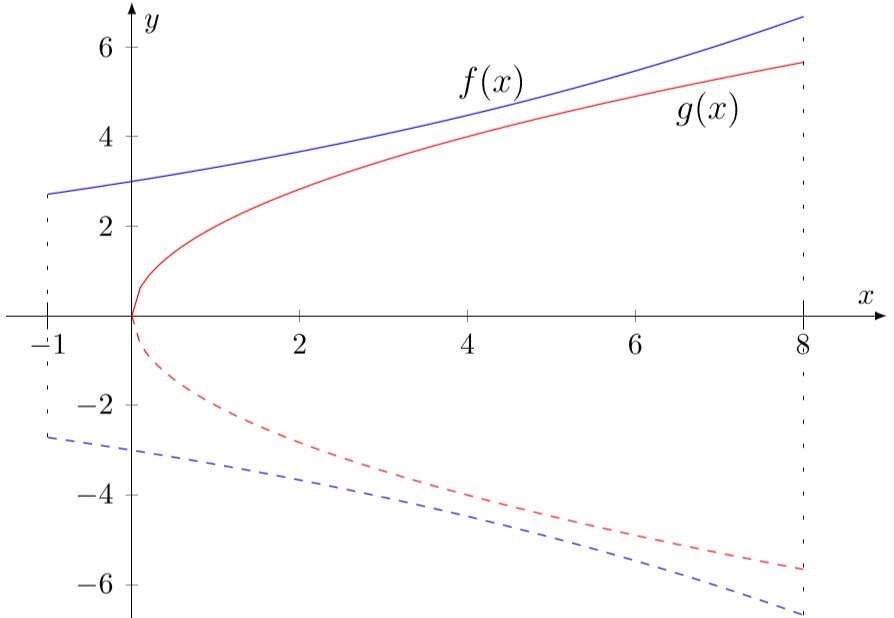
\includegraphics[scale=0.26]{fs2020-aufgabe-2}
    \end{center}
\end{multicols}

$V_1 = \pi \int \limits_{-1}^{8} f^2(x) \diff{x} = \pi \int \limits_{-1}^{8} (3e^{0.1x})^2 = \pi \int \limits_{-1}^{8} 9 e^{0.2x} = \pi \left[ 9 \cdot \frac{1}{0.2} e^{0.2x} \right]_{-1}^{8} = \pi (45 e^{1.6} - 45 e^{-0.2}) = 584.47$

$V_2 = \pi \int \limits_{0}^{8} g^2(x) \diff{x} = \pi \int \limits_{0}^{8} \left(2 \sqrt {x}\right)^2 \diff{x} = \pi \int \limits_{0}^{8} 4x \diff{x} = \pi \left[ 2x^2 \right]_0^8 = \pi \cdot 2 \cdot 64 = 128 \pi = 402.12$

$V = V_1 - V_2 = 584.47 - 402.12 = 182.35 \text{ cm}^3$

\textbf{b) Die Innenfläche (definiert durch die Rotation von $g(x)$ um die $x$-Achse) soll beschichtet werden.
Berechnen Sie die zu beschichtende Fläche.
Mantelfläche eines Rotationskörpers}

$g(x) = 2 \sqrt {x} \quad\quad g'(x) = 2 \cdot \frac{1}{2 \sqrt {x}} = \frac{1}{\sqrt {x}} \quad\quad (g'(x))^2 = \frac{1}{x}$
\begin{align*}
    \text{Gesamte Fläche: } M &= 2 \pi \cdot \int \limits_{0}^{8} y \cdot \sqrt {1 + (y')^2} \diff{x} = 2 \pi \int \limits_{0}^{8} 2 \sqrt {x} \cdot \sqrt {1 + \frac{1}{x}} \diff{x} = 2 \pi \int \limits_0^8 = 2 \sqrt {x + 1} \diff{x} = 4 \pi \int \limits_0^8 (x + 1)^\frac{1}{2} \diff{x} \\
    &= 4 \pi \left[ \frac{2}{3} (x + 1)^\frac{3}{2} \right]_0^8 = 4 \pi (\frac{2}{3} \cdot 9^\frac{3}{2} - \frac{2}{3}) = \frac{208\pi}{3} = 217.82 \text{ cm}^2
\end{align*}

\sssect{Aufgabe 3: Integrale und Grenzwerte}

\textbf{a) Berechnen Sie das Integral $\int \frac{\ln(x)}{x^2} \diff{x}$ mithilfe einer geeigneten Methode.}

\textbf{Partielle Integration:} $\quad u = \ln(x) \quad\quad u' = \frac{1}{x} \quad\quad v' = \frac{1}{x^2} = x^{-2} \quad\quad v = -x^{-1} = -\frac{1}{x}$

$\int \ln(x) \cdot \frac{1}{x^2} \diff{x} = uv - \int u'v = -\frac{\ln(x)}{x} + \int \frac{1}{x^2} \diff{x} = -\frac{\ln(x)}{x} + \int x^{-2} \diff{x} = -\frac{\ln(x)}{x} - \frac{1}{x} + C$

\textbf{b) Berechnen Sie das Integral $\int \limits_{1}^{\infty} \frac{\ln(x)}{x^2} \diff{x}$}

$\int \limits_{1}^{\infty} = \lim \limits_{t \to \infty} \int \limits_{1}^{t} \frac{\ln(x)}{x^2} = \lim \limits_{t \to \infty} \left( \left[ -\frac{\ln(x)}{x} - \frac{1}{x} \right]_{1}^{t} \right) = \lim \limits_{t \rightarrow \infty} \left( -\frac{\ln(t)}{t} - \frac{1}{t} - (0 - 1)\right) = 0 - 0 - (0 - 1) = 1$

\textbf{c) Bestimmen Sie den Grenzwert von $\lim \limits_{x \to 0} \frac{x}{\ln(3x + 1)}$}

Bernoulli-Hôpital mit $f(x) = x$ und $g(x) = \ln(3x + 1)$ anwenden:

$f'(x) = 1, g'(x) = \frac{1}{3x + 1} \cdot 3 = \frac{3}{3x + 1}$

$\frac{f'(x)}{g'(x)} = \frac{1}{\frac{3}{3x + 1}} = \frac{3x + 1}{3} \xrightarrow[x \to 0]{} \frac{1}{3}$

\textbf{d) Bestimmen Sie den Grenzwert von $\lim \limits_{x \to \infty} x \cdot \ln\left(\frac{x + 2}{x - 3}\right)$}

Umformen zu einem Bruch: \[x \cdot \ln\left( \frac{x + 2}{x - 3} \right) = \frac{\ln\left( \frac{x + 2}{x - 3} \right)}{1/x}\]

Bernoulli-Hôpital anwenden mit $f(x) = \ln \left( \frac{x + 2}{x - 3} \right)$ und $g(x) = \frac{1}{x}$:

$f'(x) = (\ln (x + 2) - \ln(x - 3))' = \frac{1}{x + 2} - \frac{1}{x - 3} = \frac{(x - 3) - (x + 2)}{(x + 2)(x - 3)} = -\frac{5}{(x + 2)(x - 3)}$

$g'(x) = (x^{-1})' = -x^{-2} = - \frac{1}{x^2}$

$\displaystyle \lim \limits_{x \to \infty} \frac{f(x)}{g(x)} = \lim \limits_{x \to \infty} \frac{f'(x)}{g'(x)} = \lim \limits_{x \to \infty} = \frac{-\frac{5}{(x + 2)(x - 3)}}{-\frac{1}{x^2}} = \lim \limits_{x \to \infty} \frac{5x^2}{(x + 2)(x - 3)} = 5$

\newpage

\sssect{Aufgabe 4: Differentialgleichungen}

Wir betrachten die Differentialgleichung \[y' \cdot y = x - 1\]

\begin{multicols}{2}
    \textbf{a) Bestimmen Sie die allgemeine Lösung.}

    $y' \cdot y = x - 1 \Rightarrow y' = \frac{x - 1}{y}$

    Separierbare DGL mit $f(x) = x - 1$ und $g(x) = \frac{1}{y}$
    \begin{align*}
        &\frac{\diff{y}}{\diff{x}} = \frac{1}{y} \cdot (x - 1) \Rightarrow \int y \cdot \diff{y} = \int (x - 1) \diff{x} \\
        &\Rightarrow \frac{y^2}{2} = \frac{x^2}{2} - x + C \Rightarrow y^2 = x^2 - 2x + 2C \\
        &\Rightarrow y = \pm \sqrt {x^2 - 2x + 2C}
    \end{align*}

    \columnbreak

    \textbf{b) Bestimmen Sie die Lösung zum Anfangswert $y(0) = 5$ und berechnen Sie den exakten Funktionswert $y(2)$}

    Da $y(0) = 5 > 0$ muss das Vorzeichen positiv sein.

    $x = 0$ und $y = 5$ einsetzen: $5 = \sqrt {0 - 0 + 2C} \Rightarrow 25 = 2C \Rightarrow C = 12.5$

    Somit: $y = \sqrt {x^2 - 2x + 25}$

    $y(2) = \sqrt {2^2 - 2 \cdot 2 + 25} = 5$
\end{multicols}

\textbf{c) Wir betrachten die obige DGL mit der Anfangsbedingung $y(0) = 5$.
Führen Sie zwei Euler-Schritte mit einer Schrittweite von $h = 1$ hintereinander durch, um den zugehörigen \emph{Schätzwert} für den Funktionswert bei $x = 2$ zu erhalten.}

$x_0 = 0, y_0 = 5, h = 1, F(x,y) = \frac{x-1}{y}$

\begin{multicols}{2}
    1. Euler-Schritt:
    \begin{align*}
        x_1 &= x_0 + h = 1 \\
        y_1 &= y_0 + h \cdot F(x_0, y_0) = 5 + 1 \cdot \frac{0 - 1}{5} = 4.8
    \end{align*}

    2. Euler-Schritt:
    \begin{align*}
        x_2 &= x_1 + h = 2 \\
        y_2 &= y_1 + h \cdot F(x_1, y_1) = 4.8 + 1 \cdot \frac{1 - 1}{4.8} = 4.8
    \end{align*}
\end{multicols}

\sssect{Aufgabe 5: Taylor-Reihen}

\textbf{a) Bestimmen Sie das Taylor-Polynom für die Funktion $f(x) = x \cdot e^x$ vom Grad $5$ um $x_0 = 0$.}

Taylor-Reihe von $e^x$ (Papula): $\displaystyle 1 + x + \frac{x^2}{2!} + \frac{x^3}{3!} + \frac{x^4}{4!} + \dots$

Taylor-Reihe von $x \cdot e^x$: $\displaystyle x \left( 1 + x + \frac{x^2}{2!} + \frac{x^3}{3!} + \frac{x^4}{4!} + \dots \right) = x + x^2 + \frac{x^3}{2!} + \frac{x^4}{3!} + \frac{x^5}{4!} + \dots$

Somit ist das gesuchte Polynom vom Grad $5$: $x + x^2 + \frac{x^3}{2} + \frac{x^4}{6} + \frac{x^5}{24}$

\textbf{b) Bestimmen Sie das Taylor-Polynom für die Funktion $g(x) = \ln(\sin(x))$ vom Grad $2$ um $x_0 = \frac{\pi}{2}$}

$\displaystyle g(x) = \ln(\sin(x)) \quad\quad g'(x) = \frac{1}{\sin(x)} \cdot \cos(x) \quad\quad g''(x) = \frac{-\sin(x) \cdot \sin(x) - \cos(x) \cdot \cos(x)}{\sin^2(x)}$

$\displaystyle g(x_0) = \ln(1) = 0 \quad\quad g'(x_0) = \frac{\cos(\pi / 2)}{\sin(\pi / 2)} = 0 \quad\quad g''(x_0) = \frac{-1}{1} = -1$

Gesuchtes Polynom:
\begin{align*}
    p_2(x) &= g(x_0) + g'(x_0) \cdot (x - x_0) + \frac{g''(x_0)}{2} \cdot (x - x_0)^2 \\
    &= 0 + 0 - \frac{1}{2} \cdot (x - \pi/2)^2 = -\frac{1}{2} (x - \pi/2)^2
\end{align*}

\textbf{c) Bestimmen Sie den Konvergenzradius der Potenzreihe $\displaystyle p(x) = \sum \limits_{k=0}^{\infty} \left( \frac{4^k}{k^2} \cdot x^k \right)$}

$\displaystyle p(x) = \sum \limits_{k=0}^{\infty} a_k \cdot (x - x_0)^k = \sum \limits_{k=0}^{\infty} \left( \frac{4^k}{k^2} \cdot x^k \right)$ mit $a_k = \frac{4^k}{k^2}$

Konvergenzradius:
$\displaystyle \lim \limits_{k \to \infty} \left| \frac{a_k}{a_{k+1}} \right| = \lim \limits_{k \to \infty} \frac{\frac{4^k}{k^2}}{\frac{4^{k+1}}{(k+1)^2}} = \lim \limits_{k \to \infty} \frac{4^k \cdot (k+1)^2}{4^{k+1} \cdot k^2} = \lim \limits_{k \to \infty} \frac{1 \cdot (k + 1)^2}{4 \cdot k^2} = \lim \limits_{k \to \infty} \frac{1}{4} \cdot \frac{(k+1)^2}{k^2} \xrightarrow[k \to \infty]{} \frac{1}{4} \cdot 1 = \frac{1}{4}$

\sssect{Aufgabe 6: Differentialgleichungen und Taylor-Reihen}

\textbf{a) Wir betrachten die DGL}
\[y' = 3 \sin(x) \cdot e^{-x^3} - 3x^2 \cdot y\]
\textbf{Bestimmen Sie die allgemeine Lösung der obigen DGL}

Umformen ergibt: $y' + \overbrace{3x^2 \cdot y}^{f(x)} = \overbrace{3 \sin(x) \cdot e^{-x^3}}^{g(x)}$

Es ist also eine lineare Differentialgleichung von der Form: $y' + f(x) \cdot y = g(x)$ mit $f(x) = 3x^2$ und $g(x) = 3\sin(x) \cdot e^{-x^3}$.

Gemäss Rezept: $F(x) = x^3$ und $y_0 = C \cdot e^{-F(x)} = C \cdot e^{-x^3}$

Somit ist $K(x) = \int g(x) \cdot e^{-F(x)} \diff{x} = \int 3 \sin(x) \cdot e^{-x^3} \cdot e^{x^3} \diff{x} = \int 3 \sin(x) \diff{x} = -3 \cos(x) + C$

Schlussendlich: $y = (-3 \cos(x) + C) \cdot e^{-x^3}$

\textbf{b) Bestimmen Sie den Konvergenzradius der Potenzreihe} $\displaystyle p(x) = \sum \limits_{k = 0}^{\infty} \frac{(2x + 1)^k}{3^k}$

Umformen ergibt:
\[\sum \limits_{k=0}^\infty \frac{(2x + 1)^k}{3^k} = \sum \limits_{k=0}^\infty \frac{(2(x + 0.5))^k}{3^k} = \sum \limits_{k=0}^\infty \frac{2^k \cdot (x + 0.5)^k}{3^k} = \sum \limits_{k=0}^\infty \frac{2^k}{3^k} \cdot (x + 0.5)^k\]

Also ist $\displaystyle a_k = \frac{2^k}{3^k} = \left( \frac{2}{3} \right)^k$

Somit ist der Konvergenzradius: $\displaystyle \lim \limits_{x \to \infty} \left| \frac{a_k}{a_{k+1}} \right| = \lim \limits_{x \to \infty} \frac{(2/3)^k}{(2/3)^{k+1}} = \lim \limits_{x \to \infty} \frac{1}{2/3} = \frac{3}{2}$
\end{document}